% !TEX root = ../Tesis.tex
\chapter{Descomposición de señales} % Write in your own chapter title
\label{cap:desc} 

%\texttt{nocite} \nocite{DWT-NARNN}

Una serie de tiempo, en el ámbito financiero, se entiende como una sucesión de datos ordenados cronológicamente que, en el caso de nuestro estudio, representan el precio de las acciones. Presentan fluctuaciones importantes, pues el valor en el mercado de estos instrumentos en un espacio de tiempo corto, digamos de 2 semanas, puede parecer ir a la alza, hasta que algún factor externo actué sobre él e interrumpa su curso. Estas perturbaciones en la tendencia hacen difícil generar una observación de los patrones que la componen y aún más si tratamos el problema desde un análisis frecuencial, pero, como veremos a lo largo del capítulo, no es difícil llegar a estos resultados usando las técnicas adecuadas.

\section{Transformada de Fourier (FT)}

Dentro del campo del procesamiento de señales una de las técnicas más populares en su análisis es sin duda la Transformada de Fourier (\textit{Fourier Transform}) (TF):

$$
F(\omega) = \frac{1}{\sqrt{2\pi}}\int_{-\infty}^{\infty} f(t) e^{-i\omega t} \, dt
$$
% Fórmula obtenida de: ten_lec_wavelets_Daubechies_1

Donde:

\begin{itemize}
  \item \( f(t) \) es la señal original en el dominio del tiempo.
  \item \( e^{-i\omega t} \) es el término de frecuencia compleja.
  \item \( t \) es la variable tiempo.
  \item \( \omega \) es la frecuencia.
\end{itemize}

 Esta herramienta nos permite conocer las frecuencias que componen una señal %periódica
% detectar los elementos de periodicidad en la señal %meter histogramas de las matrices de pesos
pasando de un dominio de intensidad contra tiempo a uno que representa su frecuencia y su magnitud. Los coeficientes resultantes representan qué tanto contribuyen las funciones base (\textit{basis functions}), senos y cosenos, a la construcción de nuestra señal original. Es precisamente por ello que, como menciona Graps, A. \citep{an_introduction_to_wavelets}, la notable desventaja de la Transformada de Fourier, es no poder ubicar temporalmente cada una de esas frecuencias. Simplemente conocemos qué funciones y cómo intervienen en la creación de la onda que estudiamos, pero no cuándo ocurren estas intervenciones.

Una solución a las limitaciones de la TF es  %ya sea en su version continua, discreta o en ventanas, es la dificultad que tiene esta en ubicar en el tiempo las frecuencias que componen la señal, haciendo dificil el análisis de una serie no estacionaria como lo es nuestro objeto de estudio.
la Transformada de Fourier de Tiempo Reducido (\textit{Short Time Fourier Transform}) (TFTR) o también llamada Transformada de Fourier por Ventanas (\textit{Windowed Fourier transform}) (WFT), pues trata a la transformada ubicándola temporalmente en un intervalo fijo en el tiempo de la señal no estacionaria en el que tratamos a ésta como si lo fuera, para así obtener el análisis frecuencial. Al momento de realizar la convolución, solo  se emplea sobre la región que delimita la función $g(t-\tau)$, como se ve:

\begin{figure}[h]
    \centering
    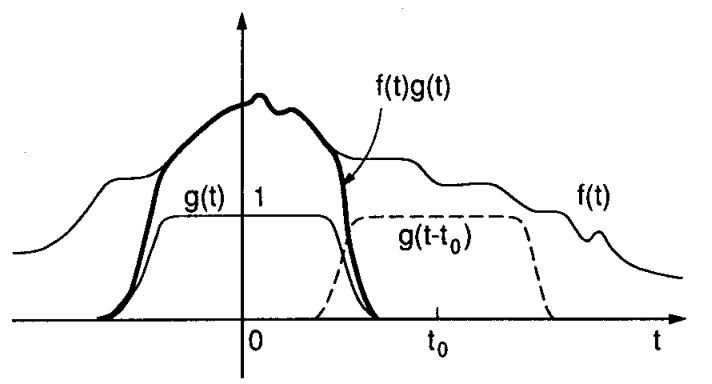
\includegraphics[width=0.5\textwidth]{Figuras/descomposicion/windowed_fourier_transform.png}
    \caption{La Transformada de Fourier de Tiempo Reducido: la función $f(t)$ es multiplicada con la función $g(t)$, obteniendo $f(t)g(t)$, repitiendo este proceso para $g(t-t_0)$, $g(t-2t_0)$ (Imagen recuperada de \cite{ten_lec_wavelets_Daubechies_1}).} 
    \label{fig:WFT}
\end{figure}

\newpage

De manera que se obtiene una descomposición temporal más detallada, se define como sigue:\\
%en deterioro de la frecuencial, pues los componentes de baja frecuencia de la onda se ven distorsionadas debido a que estas se presentan en espacios temporales amplios. 

\begin{center}

$
F(\tau, \omega) = \int_{-\infty}^{\infty} f(t) g(t - \tau) e^{-i\omega t} \, dt
$
% Fórmula obtenida de: ten_lec_wavelets_Daubechies_1
    
\end{center}


Donde \footnote{Formula recuperada de \cite{STFT}.}:

\begin{itemize}
  \item \( f(t) \) es la señal original en el dominio del tiempo.
  \item \( w(t - \tau) \) es la función de ventana que se aplica a la señal en el tiempo \( t \). Esta función de ventana suele ser una función que tiene un valor máximo en \( t \) y disminuye hacia los lados.
  \item \( e^{-i\omega t} \) es el término de frecuencia compleja.
  \item \( \omega \) es la frecuencia.
\end{itemize}

Los componentes de baja frecuencia de $f(t)$ son representados en intervalos de tiempo más grandes, por lo que el tamaño de la ventana, afecta directamente a la calidad del análisis respecto a las frecuencias que podemos rescatar: a mayor tamaño de ventana se podrá observar un mayor detalle en los componentes de baja frecuencia, caso opuesto a menor espacio de tiempo, donde las frecuencias que resulten serán más altas.

Si nos ubicamos en el plano de frecuencia contra tiempo, en el caso de la TFTR el cómo la transformación actúa es la misma para todas las locaciones pues independientemente de si tenemos una frecuencia alta o baja, el tamaño de la ventana respecto al tiempo es fijo, su relación es fija:

\begin{figure}[ht]
    \centering
    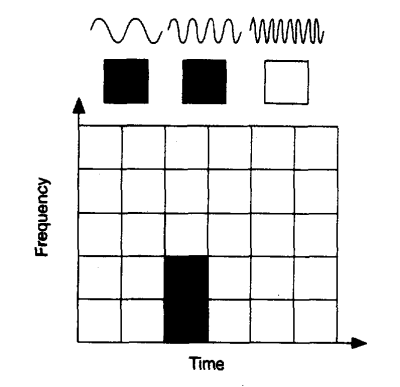
\includegraphics[width=0.5\textwidth]{Figuras/descomposicion/tiempo_frecuencia_TFTR.png}
    \caption{Plano de frecuencia contra tiempo: la manera en cómo actúa la transformación es la misma para cada ventana de tiempo, pues su tamaño es fijo e invariable para analizar cualquier frecuencia alta o baja (Recuperado de \cite{an_introduction_to_wavelets}).} 
    \label{fig:tiempo_frecuencia_TFTR}
\end{figure}

\newpage

\section{Transformada de Ondículas (WT)}

La Transformada de Ondículas o Transformada de Ondeletas (\textit{Wavelet Transform}) (WT) es una técnica avanzada en el procesamiento de señales que descompone datos o funciones en sus coeficientes de frecuencias. Depende de dos variables, la escala o frecuencia $a$ y la traslación sobre tiempo $b$, permitiendo un análisis frecuencial-temporal de la señal.

Notamos dos enfoques de Transformada de Ondículas: La Transformada Continua de Ondículas (\textit{Continuos Wavelet Transform} (CWT): 

\[
W_{f}(a, b) = \frac{1}{\sqrt{|a|}} \int_{-\infty}^{\infty} f(t) \psi^{*} \left(\frac{t-b}{a}\right) \, dt
\]

Donde:
\begin{itemize}
  \item \( f(t) \) es la función original.
  \item \( \psi^{*}(t) \) es la función conjugada compleja de \( \psi \).
  \item \( a \) y \( b \), parámetros de escala y traslación respectivamente.
\end{itemize}

Se define como la integral sobre la convolución entre nuestra señal original y una función de corta duración, que pertenece a una familia de funciones referenciadas por $a$ y $b$ que tienen la forma $\psi^{a,b}(s) = |a|^{-1/2}\psi(s-b/a)$, donde $\psi$ es llamada ondícula madre (\textit{mother wavelet}), que será nuestra función base.

Al \( \psi(t) \) comprimirse o expandirse dependiendo de $a$, $\psi^{a,0}(s)$ = $|a|^{-1/2}\psi(s/a)$ cubre diferentes rangos de frecuencia. A mayor sea el valor de $|a|$ la salida se entenderá por componentes pertenecientes a frecuencias bajas, y un valor menor de $|a|$ corresponde a frecuencias más altas. Es aquí donde surge la principal diferencia entre ésta y la TFTR, encontrando esta última una limitante en el hecho de que $g(t-\tau)$ tiene una longitud fija, lo cual acota el análisis frecuencial en cada ventana, solo $w$ puede trasladarse sobre $f(t)$ a una localización temporal adecuada:

\begin{figure}[h]
    \centering
    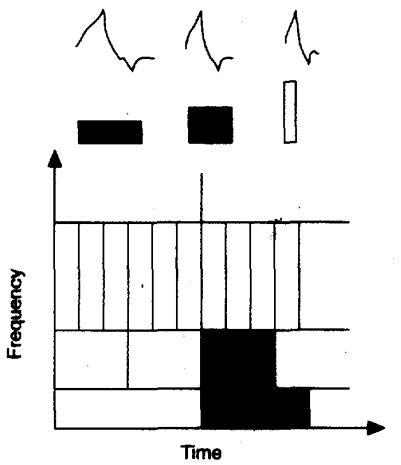
\includegraphics[width=0.5\textwidth]{Figuras/descomposicion/tiempo_frecuencia_WT.png}
    \caption{Plano de frecuencia contra tiempo: a diferencia de la TFTR, la CWT encuentra en la ampliación o compresión de $\psi^{a,b}$ la capacidad para realizar un análisis frecuencial adecuado en cada caso (Recuperado de \cite{an_introduction_to_wavelets}).} 
    \label{fig:tiempo_frecuencia_CWT}
\end{figure}

Ya que el problema que tratamos requiere el manejo de datos discretos, nos apoyaremos de la Transformada de Ondículas Discreta (\textit{Discrete Wavelet Transform}) (DWT). Se define como sigue:

\[
D_{X}(a,b) = a^{-m} \int_{-\infty}^{\infty} X(t) \psi\left( a_{0}^{-m}t-nb_{0} \right) dt
\]

Donde:
\begin{itemize}
  \item \( X(t) \) es la función original discretizada, nuestra serie de tiempo.
\end{itemize}

Típicamente, el valor de $a_0=2$ y $b_0 = 1$ para la discretización, de manera que %Donde $a=2^j$ y $b=2^jm$. 
las funciones base que son obtenidas de la ondícula madre se definen de la siguiente manera:

\[\psi_{j,k}(t) = 2^{j/2} \psi(2^{j} t - b)\]

 una familia de funciones que forman una base ortonormal para $L^2(R)$. Una de las primeras funciones $\phi$ que cumple con estos requerimientos es la función Haar, aunque en la literatura podemos encontrar otras como la función Daubechies (en la figura \ref{fig:funciones_ondículas_madre}), o la función Biortogonal.

\begin{figure}[H]
    \centering
    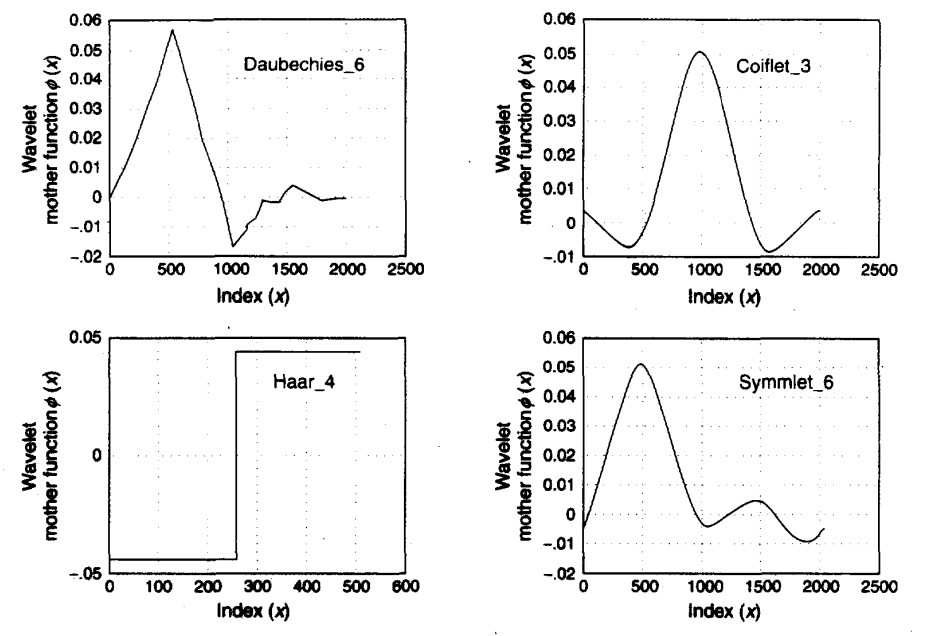
\includegraphics[width=0.5\textwidth]{Figuras/descomposicion/wavelet_mother_functions.png}
    \caption{Ejemplos de funciones de ondículas madre: Los momentos de desaparición (que se ven reflejados por el número al lado del nombre de la ondícula) se refieren a la capacidad de una ondícula para \textit{desvanecerse} al ser integrada con polinomios de cierto grado. En términos simples, si una ondícula tiene n momentos de desaparición, esto implica que el área bajo la ondícula multiplicada por un polinomio de grado n (o inferior) es igual a cero. (Recuperado de \cite{an_introduction_to_wavelets}).} 
    \label{fig:funciones_ondículas_madre}
\end{figure}

Para obtener los componente de baja y alta frecuencia de $X(t)$, la DWT usa dos conjuntos de funciones, llamadas funciones de escala (\textit{scale functions}) $\phi$ y funciones de ondícula $\psi$ (\textit{wavelet functions}) que están asociadas a un filtro de paso bajo (\textit{low-pass filter}) $\hat{g}$ y a uno de paso alto (\textit{high-pass filter}) $\hat{h}$ respectivamente. Después de filtrar los datos aplicando la transformada usando a $\psi$ y a $\phi$ como funciones base, se eliminan la mitad de los valores mediante un submuestreo, de manera que esta mitad restante caracterice las componentes bajas o altas de la señal en cada caso. Un filtro de paso bajo permite el paso de las frecuencias menores, que presentan mayor amplitud, así atenuando las características de la señal, obteniendo aquellas que representan de manera más general o suavizan a $X(t)$. Lo que obtenemos serán los coeficientes de aproximación en la resolución $2^{j}$ (\textit{Aproximation Coefficients}) ($A_{2^{j}}X$). Por otro lado, si se permite el paso de frecuencias altas o ruido presente en la señal se trata de un filtro de paso alto y se obtendrán los coeficientes de detalle en la resolución $2^{j}$ de la señal (\textit{Detail Coefficients}) ($D_{2^{j}}X$). A este procedimiento se le conoce como Codificación por Sub-bandas (\textit{Subband Coding}) \cite{wavalet_tutorial_Polizar}.

Para una descomposición superior este proceso se puede repetir, aplicando un algoritmo piramidal partiendo de los coeficientes de aproximación a un nivel de resolución $2^{j-1}$ se puede obtener los coeficientes de detalle y aproximación del nivel $2^{j}$ de manera que los coeficientes de detalle de este nivel representan las diferencias entre los coeficientes de aproximación este nivel y el anterior. Tal es el comportamiento del algoritmo de descomposición de multi-resolución propuesto por Mallat \cite{mulresolution_sigmal_desc_DWT_Mallat} como se ve reflejado en la siguiente figura:

%insertar figura del algoritmo de descomposicion de multiresolución

\begin{figure}[H]
    \centering
    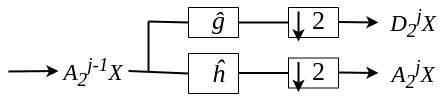
\includegraphics[width=0.5\textwidth]{Figuras/descomposicion/multiresolution_analisis_DWT.png}
    \caption{Descomposición de los componentes de aproximación $A_{2^{j-1}}X$ en sus respectivos componentes de aproximación $A_{2^{j}}X$ y de detalle $D_{2^{j}}X$, pasándolos por los filtros de paso alto y bajo $\hat{g}$ y $\hat{h}$ y aplicando un submuestreo.}
    \label{fig:algoritmo_por_subbandas}
\end{figure}

Aplicando el algoritmo de descomposición de multi-resolución a datos reales, se ve como sigue:

\begin{figure}[H]
    \centering
    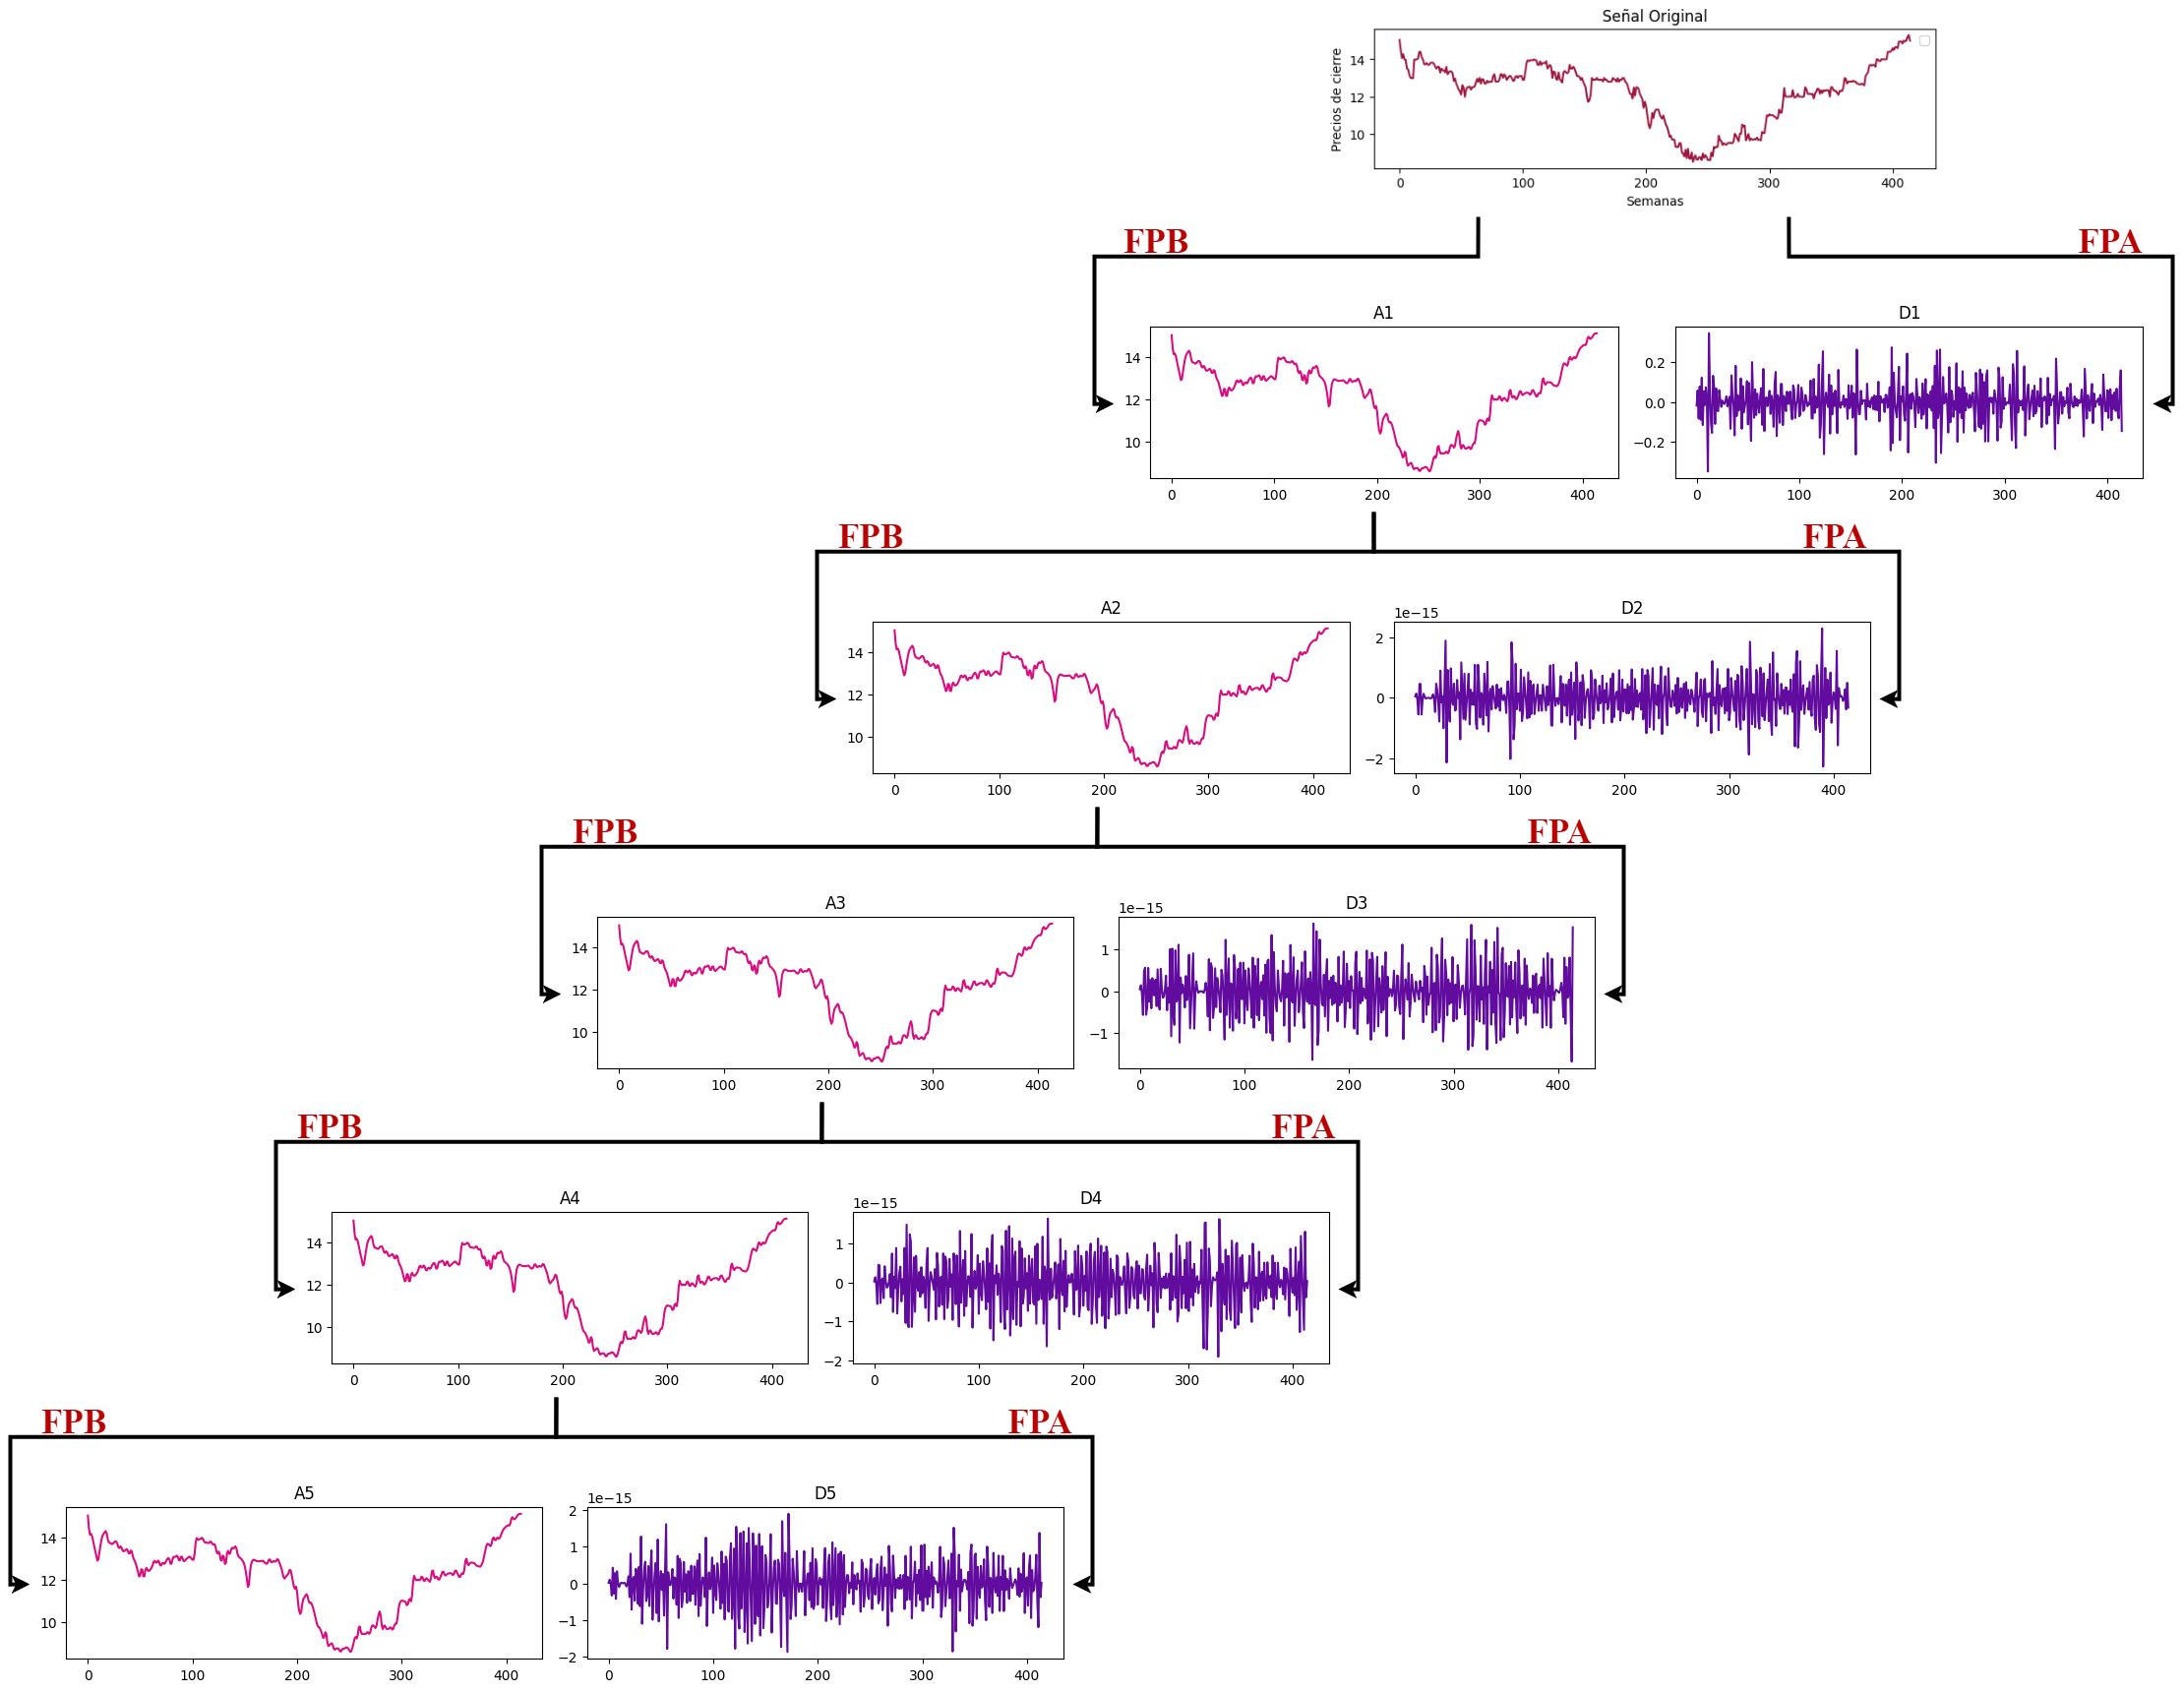
\includegraphics[width=0.9\textwidth]{Figuras/construccion_del_modelo/ACTINVRB_DWT_lvl1_5.png}
    \caption{Componentes de detalle y aproximación en cinco niveles de los datos de \textbf{ACTINVRB}.} 
    \label{fig:ACTINVRB_DWT_nivel1_5}
\end{figure}

Para la reconstrucción, las señales son aumentadas (\textit{upsampled}) por un factor de dos, pasadas por los filtros de síntesis $h[n]$ de paso bajo y $g[n]$ de paso alto y luego simplemente sumando para obtener la reconstrucción en una resolución anterior. Es a este nivel, donde trabajaremos con nuestra serie de tiempo.

\begin{figure}[H]
    \centering
    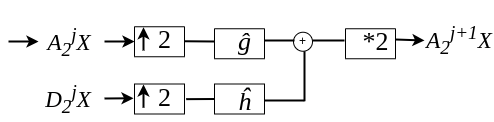
\includegraphics[width=0.5\textwidth]{Figuras/descomposicion/Recomposition_DWT.png}
    \caption{Reconstrucción de los componentes de aproximación $A_{2^{j+1}}X$ a partir de sus componentes de aproximación $A_{2^{j}}X$ y de detalle $D_{2^{j}}X$, pasándolos por los filtros de síntesis de paso alto y bajo $g$ y $h$ y aplicando un muestreo ascendente.}
    \label{fig:reconstruccion_DWT}
\end{figure}




%Desarrollo de las ondículas

